%% Dexter Barrows, 2016
%% dbarrows.github.io

\section{Intro}

    Markov Chain Monte Carlo (MCMC) is part of a general class of methods designed to sample from the posterior distribution of model parameters. It is an algorithm used when we wish to fit a model $M$ that depends on some parameter (or more typically vector of parameters) $\theta$ to observed data $D$. MCMC works by constructing a Markov Chain whose stationary or equilibrium distribution is used to approximate the desired posterior distribution.


\section{Markov Chains}

    Consider a finite state machine with 3 states $S = \{x_1, x_2, x_3\}$, where the probability of transitioning from one particular state to another is shown as a transition graph in Figure [\ref{fsm}]. 

    \begin{figure}
        \centering
        \captionsetup{width=0.8\linewidth}
        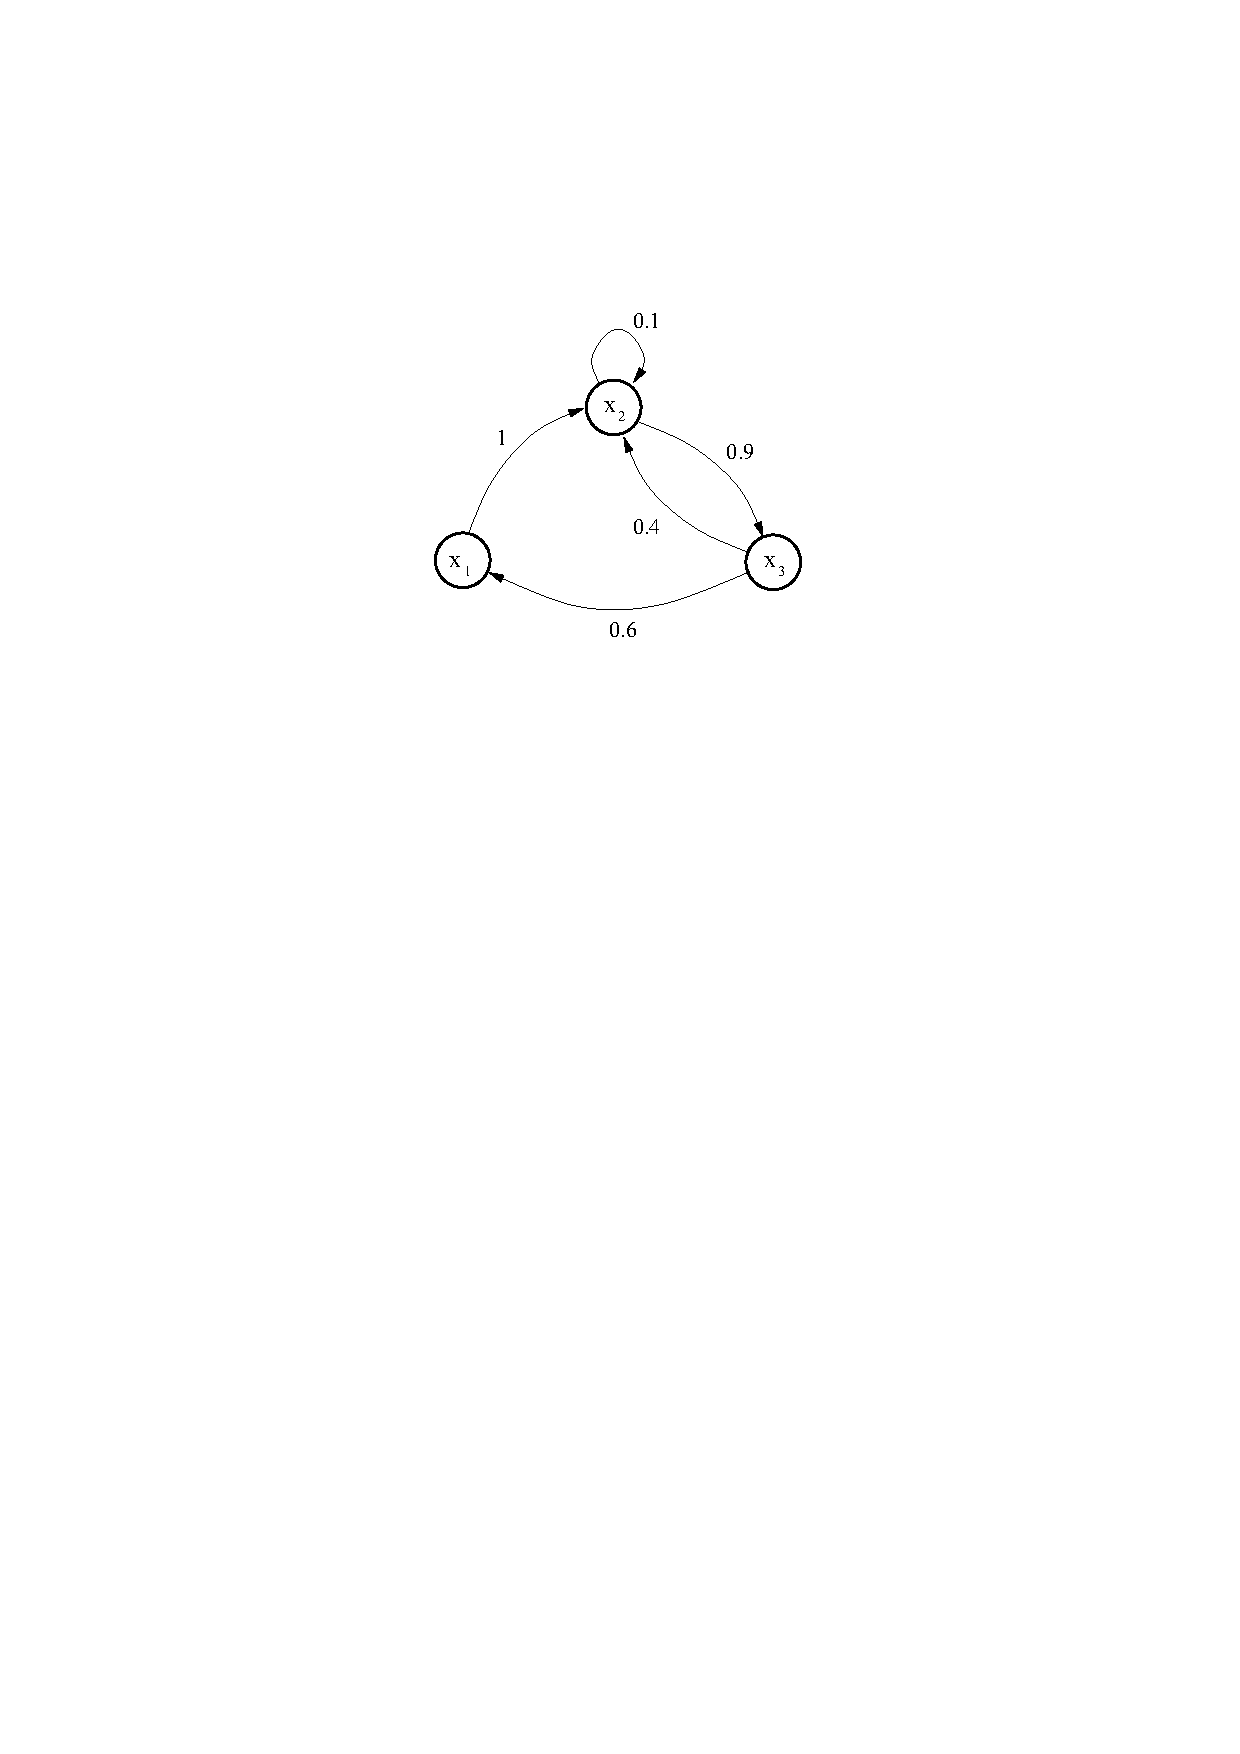
\includegraphics[width=0.5\textwidth]{./images/finitemachine.pdf}
        \caption{Finite state machine. \textit{(Andrieu et al., 2003)} \label{fsm}}
    \end{figure}

    The transition probabilities can be summarized as a matrix as

    $$
    T = 
    \begin{bmatrix}
        0 & 1 & 0 \\
        0 & 0.1 & 0.9 \\
        0.6 & 0.4 & 0
    \end{bmatrix}.
    $$

    The probability vector $\mu(x^{(1)})$ for a state $x^{(1)}$ can be evolved using $T$ by evaluating $\mu(x^{(1)})T$, then again by evaluating $\mu(x^{(1)})T^2$, and so on. If we take the limit as the number of transitions approaches infinity, we find

    $$
        \lim_{t \to \infty} \mu(x^{(1)})T^t = (27/122, 50/122, 45/122).
    $$

    This indicates that no matter what we pick for the initial probability distribution $\mu(x^{(1)})$, the chain will always stabilize at the equilibrium distribution.

    Note that this property holds when the chain satisfies the following conditions

    \begin{itemize}
        \item \textit{Irreducible} Any state A can be reached from any other state B with non-zero probability
        \item \textit{Positive Recurrent} The number of steps required for the chain to reach state A from state B must be finite
        \item \textit{Aperiodic} The chain must be able to explore the parameter space without becoming trapped in a cycle
    \end{itemize}

    Note that MCMC sampling generates a Markov chain $(\theta^{(1)}, \theta^{(2)},..., \theta^{(N)})$ that does indeed satisfy these conditions, and uses the chain's equilibrium distribution to approximate the posterior distribution of the parameter space.    


\section{Likelihood}

    MCMC and similar methods hinge on the idea that the weight or support bestowed upon a particular set of parameters $\theta$ should be proportional to the probability of observing the data $D$ given the model output using that set of parameters $M(\theta)$. In order to do this we need a way to evaluate whether or not $M(\theta)$ is a good fit for $D$; this is done by specifying a likelihood function $\mathcal{L}(\theta)$ such that

    $$
        \mathcal{L}(\theta) \propto P(D|\theta).
    $$

    In standard Maximum Likelihood approaches, $\mathcal{L}(\theta)$ is searched to find a value of $\theta$ that maximizes $\mathcal{L}(\theta)$, then this $\theta$ is taken to be the most likely true value. Here our aim is to not just maximize the likelihood but to also explore the area around it.


\section{Prior distribution}

    Another significant component of MCMC is the user-specified prior distribution for $\theta$ or distributions for the individual components of $\theta$ (Priors). Priors serve as a way for us to tell the MCMC algorithm what we think consist of good values for the parameters.

    Note that if very little is known about the parameters, or we are worried about biasing our estimate of the posterior, we can simply use a a wide uniform distribution. However, this handicaps the algorithm in two ways: convergence of the chain may become exceedingly slow, and more pressure is put on the likelihood function to be as good as possible -- it will now be the only thing informing the algorithm of what constitutes a ``good'' set of parameters, and what should be considered poor.


\section{Proposal distribution}

    As part of the MCMC algorithm, when we find a state in the parameter space that is accepted as part of the Markov chain construction process, we need a good way of generating a good next step to try. Unlike basic rejection sampling in which we would just randomly sample from our prior distribution, MCMC attempts to optimise our choices by choosing a step that is close enough to the last accepted step so as to stand a decent chance of also being accepted, but far enough away that it doesn't get ``trapped'' in a particular region of the parameter space.

    This is done through the use of a proposal or candidate distribution. This will usually be a distribution centred around our last accepted step and with a dispersion potential narrower than that of out prior distribution.

    Choice of this distribution is theoretically not of the utmost importance, but in practice becomes important so as to not waste computer time.


\section{Algorithm}

    Now that we have all the pieces necessary, we can discuss the details of the MCMC algorithm.

    We will denote the previously discussed quantities as

    \begin{itemize}
        \item $p(\cdot)$ - the prior distribution
        \item $q(\cdot|\cdot)$ - the proposal distribution
        \item $\mathcal{L}(\cdot)$ - the Likelihood function
        \item $\mathcal{U}(\cdot,\cdot)$ - the uniform distribution
    \end{itemize}

    and the define the acceptance ratio, $r$, as

    $$
        r = \frac{\mathcal{L}(\theta^*)p(\theta^*)q(\theta^*|\theta)}{\mathcal{L}(\theta)p(\theta)q(\theta|\theta^*)},
    $$

    where $\theta^*$ is the proposed sample to draw from the posterior, and $\theta$ is the last accepted sample.

    In the special case of the Metropolis Hastings variation of MCMC, the proposal distribution is symmetric, meaning $q(\theta^*|\theta) = q(\theta|\theta^*)$, and so the acceptance ratio simplifies to

    $$
        r = \frac{\mathcal{L}(\theta^*)p(\theta^*)}{\mathcal{L}(\theta)p(\theta)}.
    $$

    Thus, the MCMC algorithm shown in Algorithm [\ref{mhmcmc}].
    
    \begin{algorithm}

        \BlankLine

        \SetKwInOut{Input}{Input}
        \SetKwInOut{Output}{Output}
        \DontPrintSemicolon

        \tcc{Select a starting point}
        \Input{Initialize $\theta^{(1)}$}

        \BlankLine

        \For{$i = 2:N$}{

            \BlankLine

            \tcc{Sample}
            $\theta^* \sim q(\cdot|\theta^{(i-1)})$ \;
            $u \sim \mathcal{U}(0,1)$

            \BlankLine

            \tcc{Evaluate acceptance ratio}
            $r$ $\gets$ $\frac{\mathcal{L}(\theta^*)p(\theta^*)}{\mathcal{L}(\theta)p(\theta)}$

            \BlankLine

            \tcc{Step acceptance criterion}
            \eIf{ $u < \min\left\{ 1 , r \right\}$ }{ 
                $\theta^{(i)} = \theta^*$\;
            }{
                $\theta^{(i)} = \theta^{(i-1)}$\;
            }
        }

        \BlankLine

        \tcc{Samples from approximated posterior distribution}
        \Output{Chain of samples $(\theta^{(1)},\theta^{(2)},...,\theta^{(N)})$}

        \BlankLine

        \caption{Metropolis-Hastings MCMC \label{mhmcmc}}

    \end{algorithm}
    

    In this way we are ensuring that steps that lead to better likelihood outcomes are likely to be accepted, but steps that do not will not be accepted as frequently. Note that these less ``advantageous'' moves will still occur but that this is by design -- it ensures that as much of the parameter space as possible will be explored but more efficiently than using pure brute force.


\section{Burn-in}

    One critical aspect of MCMC-based algorithms has yet to be discussed. The algorithm requires an initial starting point $\theta$ to be selected, but as the proposal distribution is supposed to restrict moves to an area close to the last accepted state, then the posterior distribution will be biased towards this starting point. This issue is avoided through the use of a Burn-in period.

    Burning in a chain is the act of running the MCMC algorithm normally without saving first $M$ samples. As we are seeking a chain of length $N$, the total computation will be equivalent to generating a chain of length $M+N$.


\section{Thinning}

    Some models will require very long chains to get a good approximation of the posterior, which will consequently require a non-trivial amount of computer storage. One way to reduce the burden of storing so many samples is by thinning. This involves saving only every $n^{th}$ step, which should still give a decent approximate of the posterior (since the chain has time to explore a large portion of the parameter space), but require less room to store.


\section{Hamiltonian Monte Carlo}

    The Metropolis-Hastings algorithm has a primary drawback in that the parameter space may not be explored efficiently -- a consequence of the rudimentary proposal mechanism. Instead, smarter moves can be proposed through the use of Hamiltonian dynamics, leading to a better exploration of the target distribution and a decrease in overall computational complexity.

    From physics, we will borrow the ideas of potential and kinetic energy. Here potential energy is analogous to the negative log likelihood of the parameter selection given the data, formally

    \begin{equation}
        U(\theta) = -log(\mathcal{L}(\theta)p(\theta)).
    \end{equation}

    Kinetic energy will serve as a way to ``nudge'' the parameters along a different moment for each component of $\theta$. We introduce $n$ auxiliary variables $r = (r_1, r_1,...,r_n)$, where $n$ is the number of components in $\theta$. Note that the samples drawn for $r$ are not of interest, they are only used to inform the evolution of the Hamiltonian dynamics of the system. We can now define the kinetic energy as

    \begin{equation}
        K(r) = \frac{1}{2} r^T M^{-1} r,
    \end{equation}

    where $M$ is an $n \times n$ matrix. In practice $M$ can simply be chosen as the identity matrix of size $n$, however it can also be used to account for correlation between components of $\theta$.

    The Hamiltonian of the system is defined as

    \begin{equation}
        H(\theta,r) = U(\theta) + K(r),
    \end{equation}

    Where the Hamiltonian dynamics of the combined system can be simulated using the following system of ODEs.

    \begin{equation}
        \begin{array}{rl}
        \displaystyle
            \dfrac{d\theta}{dt} & = M^{-1} r \\
            \dfrac{dr}{dt} & = - \nabla U(\theta)
        \end{array}
    \end{equation}.

    It is tempting to try to integrate this system using the standard Euler evolution scheme, but in practice this leads to instability. Instead the ``Leapfrog'' scheme is used. This scheme is very similar to Euler scheme, except instead of using a fixed step size $h$ for all evolutions, a step size of $\varepsilon$ is used for most evolutions, with a half step size of $\varepsilon / 2$ for evolutions of $\frac{dr}{dt}$ at the first step, and last step $L$. In this way the evolution steps ``leapfrog'' over each other while using future values from the other set of steps, leading to the scheme's name.

    The end product of the Leapfrog steps are the new proposed parameters $(\theta^*,r^*)$. These are either accepted or rejected using a mechanism similar to that of standard Metropolis-Hastings MCMC. Now, however, the acceptance ratio $r$ is defined as

    \begin{equation}
        r = \exp \left[ H(\theta,r) - H(\theta^*,r^*) \right],
    \end{equation}

    where $(\theta,r)$ are the last values in the chain.

    Together, we have Algorithm [\ref{hmcmc}].

    \begin{algorithm}

        \BlankLine

        \SetKwInOut{Input}{Input}
        \SetKwInOut{Output}{Output}
        \DontPrintSemicolon

        \tcc{Select a starting point}
        \Input{Initialize $\theta^{(1)}$}

        \BlankLine

        \For{$i = 2:N$}{

            \BlankLine

            \tcc{Resample moments}
            \For{$i = 1:n$}{
                r(i) $\gets$ $\mathcal{N}(0,1)$
            }

            \BlankLine

            \tcc{Leapfrog initialization}
            $\theta_0$ $\gets$ $\theta^{(i-1)}$ \;
            $r_0$ $\gets$ $r - \nabla U(\theta_0) \cdot \varepsilon / 2$

            \BlankLine

            \tcc{Leapfrog intermediate steps}
            \For{$j = 1:L-1$}{
                $\theta_j$ $\gets$ $\theta_{j-1} + M^{-1} r_{j-1} \cdot \varepsilon$ \;
                $r_j$ $\gets$ $r_{j-1} - \nabla U(\theta_j) \cdot \varepsilon$
            }

            \BlankLine

            \tcc{Leapfrog last steps}
            $\theta^*$ $\gets$ $\theta_{L-1} + M^{-1} r_{L-1} \cdot \varepsilon$ \;
            $r^*$ $\gets$ $\nabla U(\theta_L) \cdot \varepsilon / 2 - r_{L-1}$            
            \BlankLine

            \tcc{Evaluate acceptance ratio}
            $r = \exp \left[ H(\theta^{(i-1)},r) - H(\theta^*,r^*) \right]$

            \BlankLine

            \tcc{Sample}
            $u \sim \mathcal{U}(0,1)$

            \BlankLine

            \tcc{Step acceptance criterion}
            \eIf{ $u < \min\left\{ 1 , r \right\}$ }{ 
                $\theta^{(i)} = \theta^*$\;
            }{
                $\theta^{(i)} = \theta^{(i-1)}$\;
            }
        }

        \BlankLine

        \tcc{Samples from approximated posterior distribution}
        \Output{Chain of samples $(\theta^{(1)},\theta^{(2)},...,\theta^{(N)})$}

        \BlankLine

        \caption{Hamiltonian MCMC \label{hmcmc}}

    \end{algorithm}

    Note that the parameters $\varepsilon$ and $L$ have to be tuned in order to maintain stability and maximize efficiency, a sometimes non-trivial process.
    

\section{Fitting}

    Here we will examine a test case in which Hamiltonian MCMC will be used to fit a Susceptible-Infected-Removed (SIR) epidemic model to mock infectious count data.

    The synthetic data was produced by taking the solution to a basic SIR ODE model, sampling it at regular intervals, and perturbing those values by adding in observation noise. The SIR model used was

    \begin{equation}
        \begin{array}{rl}
            \dfrac{dS}{dt} & = - \beta I S \\
            \dfrac{dI}{dt} & = \beta I S - rI  \\
            \dfrac{dR}{dt} & = rI
        \end{array}
    \end{equation}

    where $S$ is the number of individuals susceptible to infection, $I$ is the number of infectious individuals, $R$ is the number of recovered individuals, $\beta = R_0 r / N$ is the force of infection, $R_0$ is the number of secondary cases per infected individual, $r$ is the recovery rate, and $N$ is the population size.

    The solution to this system was obtained using the \verb|ode()| function from the \verb|deSolve| package. The required derivative array function in the format required by \verb|ode()| was specified as

    \begin{R}    
    SIR <- function(Time, State, Pars) {

        with(as.list(c(State, Pars)), {
            
            B   <- R0*r/N    # calculate Beta
            BSI <- B*S*I     # save product
            rI  <- r*I       # save product
            
            dS = -BSI       # change in Susceptible people
            dI = BSI - rI   # change in Infected people
            dR = rI         # change in Removed (recovered people)
            
            return(list(c(dS, dI, dR)))
            
        })
        
    }
    \end{R}

    The true parameter values were set to $R_0 = 3.0, r = 0.1, N = 500$ by

    \begin{R}
    pars  <- c(R0  <- 3.0,  # new infected people per infected person
              r   <- 0.1,  # recovery rate
              N   <- 500)  # population size
    \end{R}

    The system was integrated over $[0,100]$ with infected counts drawn at each integer time step. These timings were set using

    \begin{R}
    T <- 100                            # total integration time
    times <- seq(0, T, by = 1)          # times to draw solution values
    \end{R}

    The initial conditions were set to 5 infectious individuals, 495 people susceptible to infection, and no one had yet recovered from infection and been removed. These were set using

    \begin{R}
    y_ini <- c(S = 495, I = 5, R = 0)   # initial conditions
    \end{R}

    The \verb|ode()| function is called as

    \begin{R}
    odeout <- ode(y_ini, times, SIR, pars)
    \end{R}

    where \verb|odeout| is a $(T+1) \times 4$ matrix where the rows correspond to solutions at the given times (the first row is the initial condition), and the columns correspond to the solution times and S-I-R counts at those times.

    The observation error was taken to be $\varepsilon_{obs} \sim \mathcal{N}(0,\sigma)$, where individual values were drawn for each synthetic data point.

    These ``true'' values were perturbed to mimic observation error by

    \begin{R}
    set.seed(1001)  # set RNG seed for reproducibility
    sigma <- 5       # observation error standard deviation
    infec_counts_raw <- odeout[,3] + rnorm(101, 0, sigma)
    infec_counts     <- ifelse(infec_counts_raw < 0, 0, infec_counts)
    \end{R}

    where the last two lines simply set negative observations (impossible) to 0.

    Plotting the data using the \verb|ggplot2| package by

    \begin{R}
	g <- qplot(0:T, odeout[,3], geom = "line", xlab = "Time (weeks)", ylab = "Infection Count") +
		geom_point(aes(y = infec_counts)) +
		theme_bw()

	print(g)
    \end{R}

    we obtain Figure [\ref{mcmcdataplot}].

    \begin{figure}[H]
        \centering
        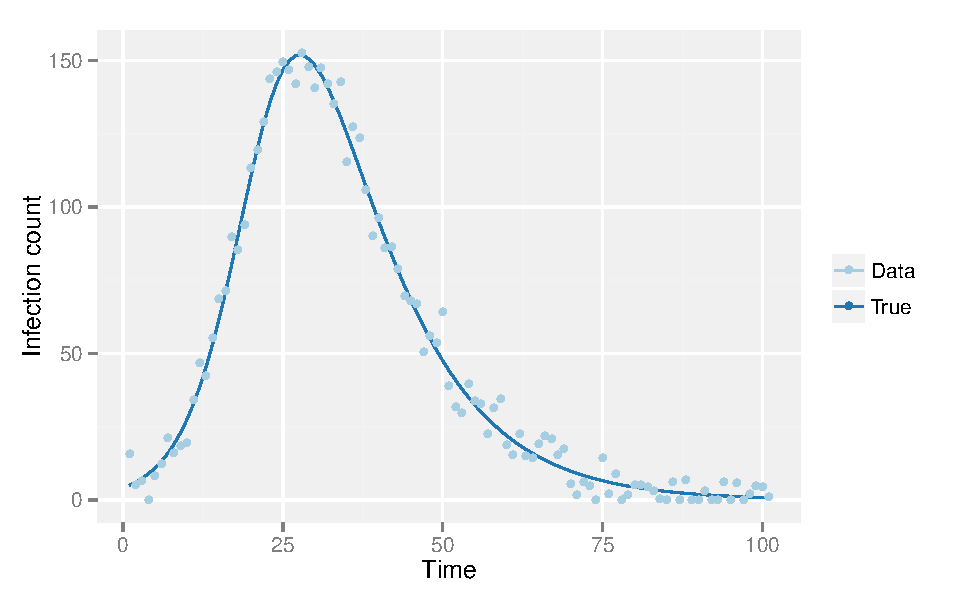
\includegraphics[width=\textwidth]{./images/dataplot.pdf}
        \caption{True SIR ODE solution infected counts, and with added observation noise}
        \label{mcmcdataplot}
    \end{figure}

    The Hamiltonian MCMC model fitting was done using Stan (\url{http://mc-stan.org/}), a program written in \verb|C++| that does Baysian statistical inference using Hamiltonian MCMC. Stan's R interface (\url{http://mc-stan.org/interfaces/rstan.html}) was used to ease implementation.

    In order to use an Explicit Euler-like stepping method in the later Stan model (both for speed and for integration method homogeneity with other methods against which HMCMC was compared), the synthetic observation counts were treated as weekly observations in which the counts on the other six days of the week were unobserved. For computational and organizational simplicity, these vales were set to -1 (all valid observations are non-negative). This is done in R using

    \begin{R}
    sPw <- 7               # steps per week
    datlen <- (T-1)*7 + 1  # size of sparse data vector

    data <- matrix(data = -1, nrow = T+1, ncol = sPw)
    data[,1] <- infec_counts
    standata <- as.vector(t(data))[1:datlen]
    \end{R}

    The data to be fed into the R Stan interface is packed as

    \begin{R}
    sir_data <- list( T = datlen,    # simulation time
                     y = standata,  # infection count data
                     N = 500,       # population size
                     h = 1/sPw )    # step size per day 
    \end{R}

    For efficiency we allow Stan to save compiled code to avoid recompilation, and allow multiple chains to be run simultaneously on separate CPU cores

    \begin{R}
    rstan_options(auto_write = TRUE)
    options(mc.cores = parallel::detectCores())
    \end{R}

    Now we call the Stan fitting function

    \begin{R}
	stan_options <- list(	  chains = 4,    # number of chains
                        	iter   = 2000, # iterations per chain
                        	warmup = 1000, # warmup interations
                        	thin   = 2 )   # thinning number
	fit <- stan( file    = "d_sirode_euler.stan",
            	data    = sir_data,
            	chains  = stan_options$chains,
            	iter    = stan_options$iter,
            	warmup  = stan_options$warmup,
            	thin    = stan_options$thin )
    \end{R}

    which fits the model in the file \verb|d_sirode_euler.stan| to the data passed in through \verb|sir_data|. The options here specify that 10 chains will be run, each with a burn in period of 1000 steps, with 5000 steps to sample over, and only sampling every 10th step. Options are saved so they can be accessed later.

    The Stan file contains three blocks that together specify the model. First, the data block specifies the information the model expects to be given. Here, this is

    \begin{Stan}
    data {

        int     <lower=1>   T;      // total integration steps
        real                y[T];   // observed number of cases
        int     <lower=1>   N;      // population size
        real                h;      // step size

    }
    \end{Stan}

    where each of the data variables correspond to data passed in through the previously shown R code.

    Next the parameters block specifies what Stan is expected to estimate. Here this is

    \begin{Stan}
    parameters {

        real <lower=0, upper=10>    sigma;  // observation error
        real <lower=0, upper=10>    R0;     // R0
        real <lower=0, upper=10>    r;      // recovery rate
        real <lower=0, upper=500>   y0[3];  // initial conditions

    }
    \end{Stan}

    Finally we have the model block. This crucial part of the code specifies the interaction between the parameters and the data. The core component of the model indicates we are fitting an approximation of an ODE model using Euler integration steps (one per day), with the initial conditions and SIR parameters unknown. Further, we can also specify the prior distributions to draw new parameter values from. The initial conditions are taken to be close to the initial data point, with adjustment for observation error, while the other parameters are assumed to be coming from log-normal distributions with relatively small means. Together, we have

    \begin{Stan}
    model {

        real S[T];
        real I[T];
        real R[T];

        S[1] <- y0[1];
        I[1] <- y0[2];
        R[1] <- y0[3];
        
        y[1] ~ normal(y0[2], sigma);

        for (t in 2:T) {

            S[t] <- S[t-1] + h*( - S[t-1]*I[t-1]*R0*r/N );
            I[t] <- I[t-1] + h*( S[t-1]*I[t-1]*R0*r/N  - I[t-1]*r );
            R[t] <- R[t-1] + h*( I[t-1]*r );
            
            if (y[t] > 0) {
                y[t] ~ normal( I[t], sigma );
            }

        }
        
        y0[1] ~ normal(N - y[1], sigma);
        y0[2] ~ normal(y[1], sigma);
        
        theta[1]    ~ lognormal(1,1);
        theta[2]    ~ lognormal(1,1);
        sigma       ~ lognormal(1,1);
            
    }
    \end{Stan}

    Examining the traceplot for the the post-warmup chain data returned by the \verb|stan()| function in the \verb|fit| object, we see that the chains are mixing well and convergence has likely been reached. This is shown in Figure [\ref{traceplot}].

    \begin{figure}
        \centering
        \captionsetup{width=0.8\linewidth}
        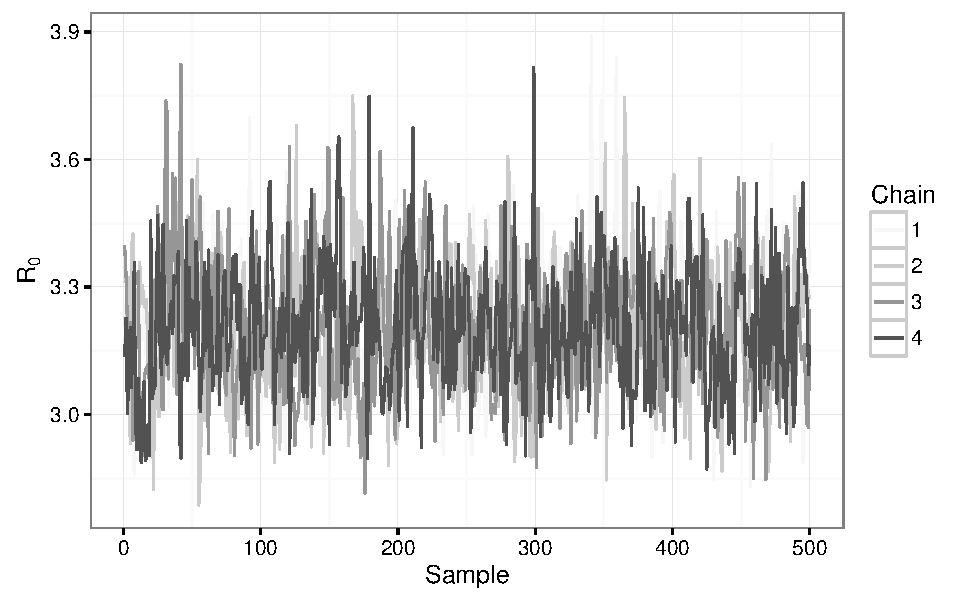
\includegraphics[width=\textwidth]{./images/traceplotR0.pdf}
        \caption{Traceplot of samples drawn for parameter $R_0$, excluding warmup \label{traceplot}}
    \end{figure}

    Further, if we look at the chain data including the warmup samples in Figure [\ref{traceplot2}], we can see why is is wise to discard these samples (note the scale).

    \begin{figure}
        \centering
        \captionsetup{width=0.8\linewidth}
        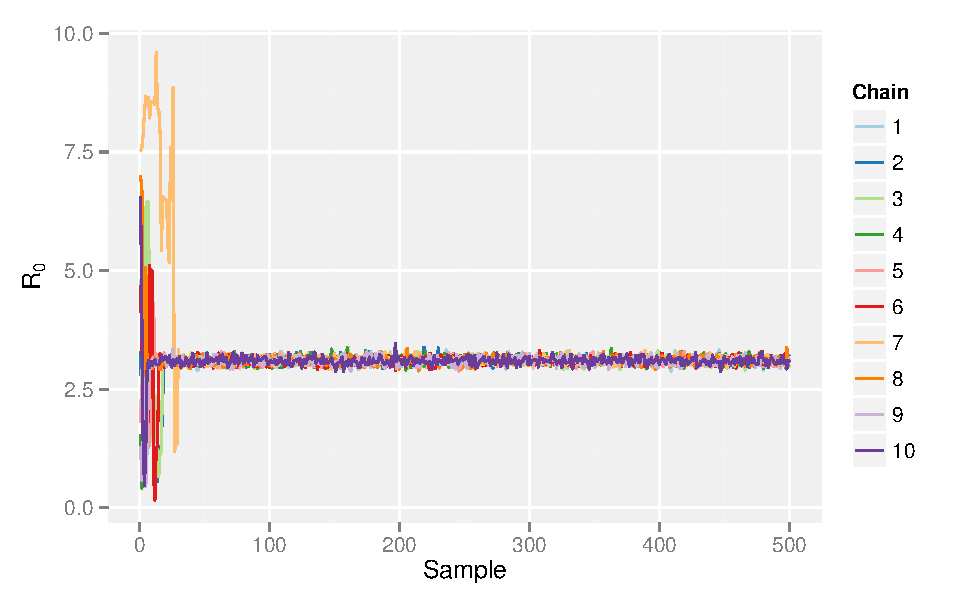
\includegraphics[width=\textwidth]{./images/traceplotR0_inc.pdf}
        \caption{Traceplot of samples drawn for parameter $R_0$, including warmup. \label{traceplot2}}
    \end{figure}

    Now if we look at the kernel density estimates for each of the model parameters and the initial number of cases, we see that while the estimates are not perfect, they are fairly decent. This is shown in Figure [\ref{hmckernels}].

    \begin{figure}
    	\centering
    	\captionsetup{width=0.8\linewidth}
        \begin{subfigure}[tl]{0.4\textwidth}
            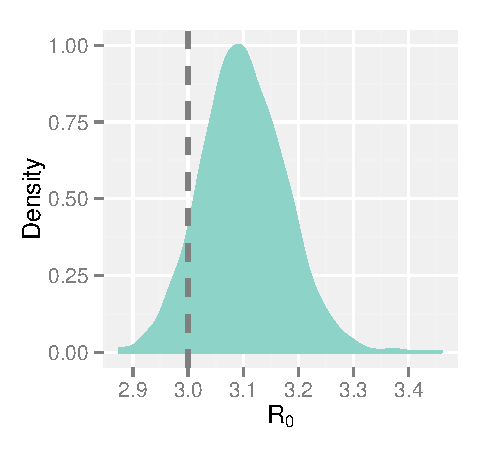
\includegraphics[width=\textwidth]{./images/kernelR0.pdf}
        \end{subfigure}
        \begin{subfigure}[tr]{0.4\textwidth}
            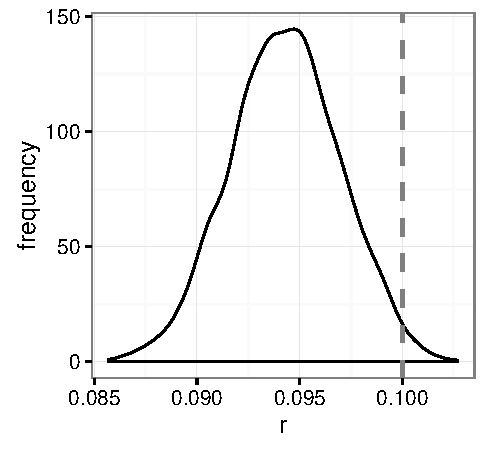
\includegraphics[width=\textwidth]{./images/kernelr.pdf}
        \end{subfigure}
        \begin{subfigure}[bl]{0.4\textwidth}
            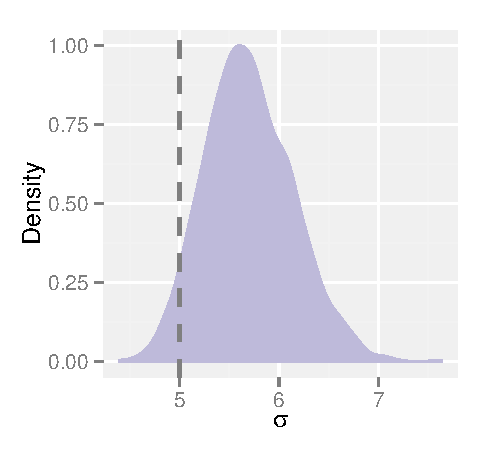
\includegraphics[width=\textwidth]{./images/kernelsigma.pdf}
        \end{subfigure}
        \begin{subfigure}[br]{0.4\textwidth}
            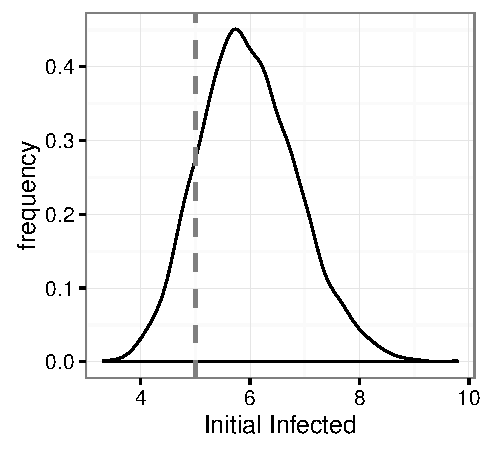
\includegraphics[width=\textwidth]{./images/kernelinfec.pdf}
        \end{subfigure}
        \caption{Kernel density estimates produced by Stan \label{hmckernels}}
    \end{figure}